 \documentclass[12pt,a4paper]{article}
\usepackage[a4paper,margin=2cm]{geometry}
\usepackage[]{graphicx}
\usepackage{bm}
\usepackage[strings]{underscore}
\usepackage{apacite}
\setlength{\parindent}{0pt}
\graphicspath{ {./images} }
\usepackage{wrapfig}
\usepackage[autostyle, english = american]{csquotes}
\usepackage[toc,page]{appendix}
\usepackage{amssymb}
\MakeOuterQuote{"}
\usepackage[T1]{fontenc}

\begin{document}
\begin{titlepage}


\title{Determining the relationship between hanging masses and the angle of a frictionless plane}

\author{Noah Alexiou}


\date{April 2025}

\maketitle
\centering

\end{titlepage}
\tableofcontents
\newpage

\section{Introduction}

\subsection{Research Question}
When the mass of an object on a frictionless plane is altered, and the mass of a hanging object adjusted so  equilibrium is achieved, can this be used to measure the angle of the plane? What is the accuracy of this method in comparison to conventional measuring techniques. 

\subsection{Rationale}

\textbf{a considered rationale for the experiment}

We noticed that when we measured the angle using the angle gun there was a lot of uncertainty. We wondered if we could utilise the inherent relationship between masses in equilibrium and the sine of the angle to measure it, and how it would compare to traditional trigonometric techniques.



\subsubsection{Hypothesis/Research Question???}
\textbf{a specific and relevant research question}

\subsection{Methodology}

\subsubsection{Modifications}


\subsubsection{Materials}
\begin{itemize}
	\item Angle gun 
	\item Frictionless plane
	\item Brass weights
	\item Blue tack 
	\item Scale
	\item Carriage
\end{itemize}

\subsubsection{Method}
\begin{enumerate}
\item Set up slope at a constant angle. It will remain at this angle for the entire duration of the experiment. 
\item Set the hanging mass for the respective set of trials $(h_m)$. 
\item Alter the cart mass $(c_m)$ until equilibrium with $h$ is achieved.
\item Measure and record masses. 
\item Increase the hanging mass by 50 grams. 
\item Repeat for set number of trials and $h_m$ values.
	
	 
\end{enumerate}


\subsubsection{Risk Assessment}
Frictionless plane
\begin{itemize}
	\item Mishandling of heavy masses on the frictionless plane could result in them sliding down the slope at high speed. This could damage equipment of cause injury. The slope will be turned off not required, and one person will always be supporting the cart whenever possible to prevent this. 
	\item Using too low fan speed on the frictionless plane may not create enough of an air pocket to support heavy weights. This could cause rubbing between the surfaces which could damage both the plane and carriage. The plane will be set to the highest possible speed throughout the experiment to negate the possibility of this occurring.
\end{itemize}
Masses
\begin{itemize}
	\item Heavy masses or items containing many brass weights may cause injury if dropped or mishandled. participants will wear enclosed footwear to negate injury if this occurs.  
\end{itemize}
\section{Results and Evaluation}
\subsection{Results}
\begin{itemize}
\item  appropriate application of algorithms, visual and graphical representations of data about linear motion and force or gravity and motion
demonstrated by correct and relevant processing of data



Data was plotted in excel, with $c$ on the $x$-axis, and  $h$ on the $y$-axis.
\begin{figure}[h]
	\centering
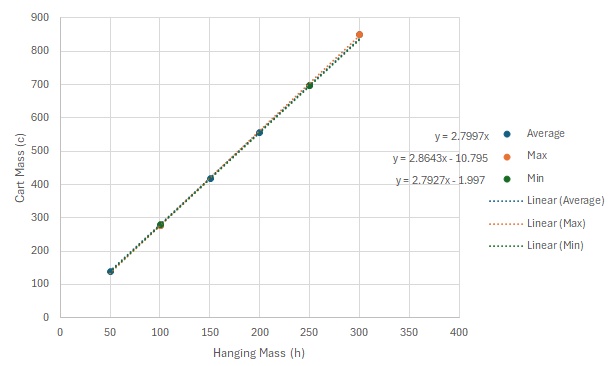
\includegraphics[width=0.8\paperwidth]{results.png}
\caption{Plot of results}
\end{figure}



\item systematic and effective analysis of experimental evidence about linear motion and force or gravity and motion demonstrated by
\begin{itemize}
	\item thorough identification of relevant trends , patterns or relationships.

What this revealed immediately is that the relationship between $h$ and $c$ was linear. Any linear relationship can be described using the formula $y=mx+c$. Clearly in this case the equation described in the graph should be $c=h\cdot m + c$.

	In theory, the data should have represented the equation:
	$$c=h\frac{1}{\sin(\theta)}$$
	which was rearranged to give 
	$$\frac{h}{c}=\sin{(\theta)}$$
	$$\frac{c}{h}=\mathrm{gradient}$$
	$$\therefore \frac{h}{c}=\frac{1}{\mathrm{gradient}}$$
	$$\therefore \sin(\theta)=\frac{1}{\textrm{gradient}}$$
	$$\therefore \sin^{-1}\left(\frac{1}{
		\textrm{gradient}}\right)=\theta$$
	
	
	
	\item thorough and appropriate identification of the uncertainty and limitations of evidence
	
	
	
	
	
	\item effective and efficient investigation of phenomena associated with linear motion and force or gravity and motion demonstrated by the collection of sufficient and relevant raw data
\end{itemize}
\end{itemize}



\subsection{Discussion}


\section{Conclusion}

	
	
	
\end{document}